\documentclass{standalone}
\usepackage{tikz}
\usetikzlibrary{patterns}
\usetikzlibrary{positioning}
\usetikzlibrary{patterns, positioning}
\usetikzlibrary{shapes.misc}
\usepackage[outline]{contour}
\contourlength{1.5pt} 


\begin{document}
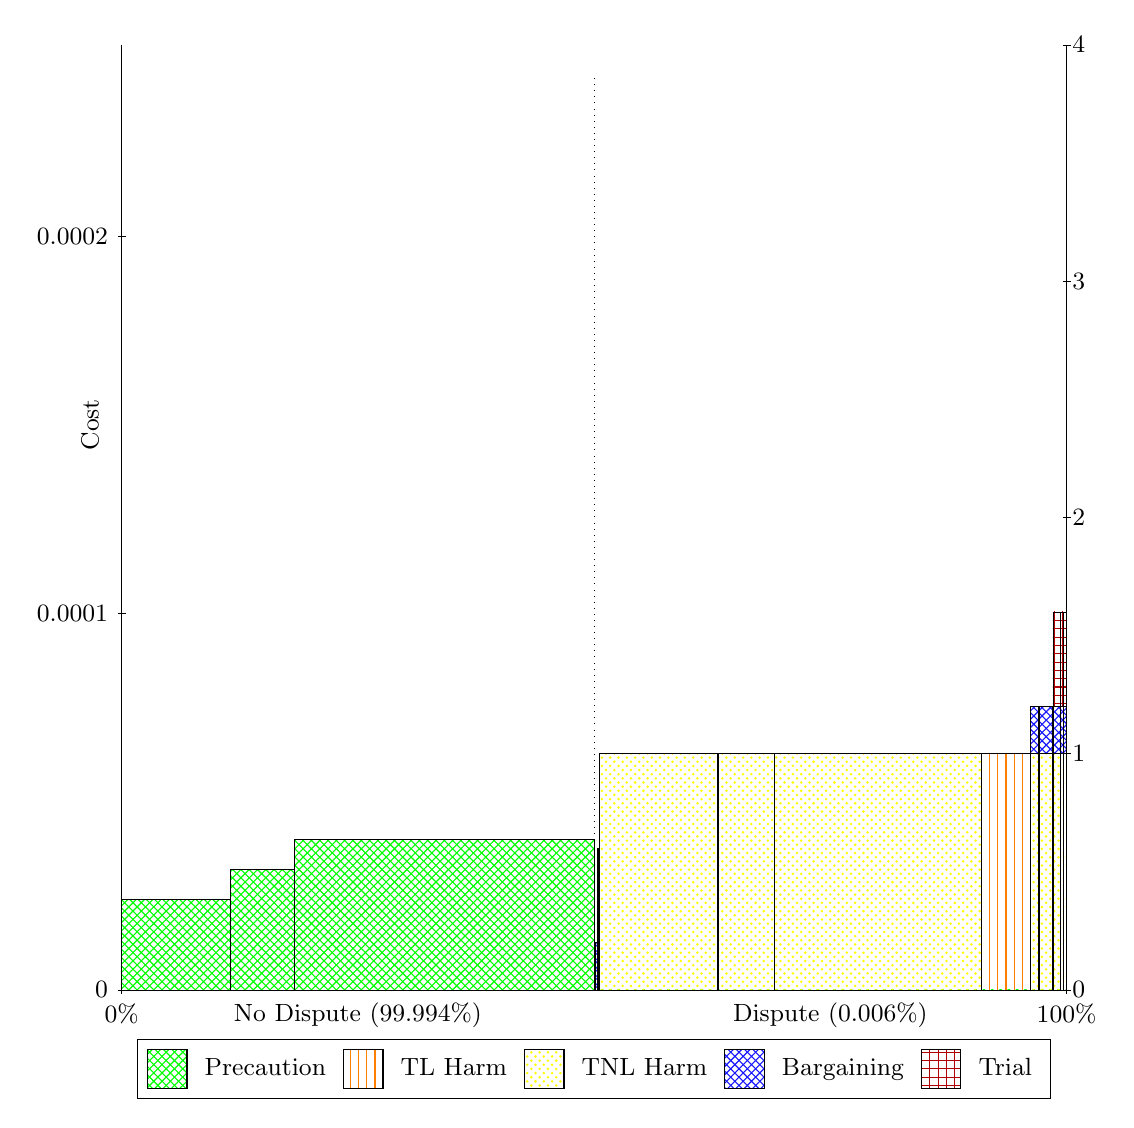
\begin{tikzpicture}
\draw[pattern=crosshatch, pattern color=green,draw=black,very thin] (1.5,2.5) rectangle (2.8801,3.6481);
\draw[pattern=crosshatch, pattern color=green,draw=black,very thin] (2.8801,2.5) rectangle (3.6907,4.0308);
\draw[pattern=crosshatch, pattern color=green,draw=black,very thin] (3.6907,2.5) rectangle (7.5,4.4135);
\draw[pattern=crosshatch, pattern color=green,draw=black,very thin] (7.5,2.5) rectangle (7.5156,2.5001);
\draw[pattern=crosshatch,      pattern color=blue!90,draw=black,very thin] (7.5,2.5001) rectangle (7.5156,3.1001);
\draw[pattern=crosshatch, pattern color=green,draw=black,very thin] (7.5156,2.5) rectangle (7.5413,2.5001);
\draw[pattern=crosshatch,      pattern color=blue!90,draw=black,very thin] (7.5156,2.5001) rectangle (7.5413,3.1001);
\draw[pattern=crosshatch, pattern color=green,draw=black,very thin] (7.5413,2.5) rectangle (7.5583,2.5001);
\draw[pattern=crosshatch,      pattern color=blue!90,draw=black,very thin] (7.5413,2.5001) rectangle (7.5583,3.1001);
\draw[pattern=grid,            pattern color=red!70!black,draw=black,very thin] (7.5413,3.1001) rectangle (7.5583,4.3001);
\draw[pattern=crosshatch, pattern color=green,draw=black,very thin] (7.5583,2.5) rectangle (7.5657,2.5001);
\draw[pattern=crosshatch,      pattern color=blue!90,draw=black,very thin] (7.5583,2.5001) rectangle (7.5657,3.1001);
\draw[pattern=grid,            pattern color=red!70!black,draw=black,very thin] (7.5583,3.1001) rectangle (7.5657,4.3001);
\draw[pattern=crosshatch, pattern color=green,draw=black,very thin] (7.5657,2.5) rectangle (9.0651,2.5001);
\draw[pattern=crosshatch dots, pattern color=yellow,draw=black,very thin] (7.5657,2.5001) rectangle (9.0651,5.5001);
\draw[pattern=crosshatch, pattern color=green,draw=black,very thin] (9.0651,2.5) rectangle (9.0815,2.5001);
\draw[pattern=vertical lines, pattern color=orange,draw=black,very thin] (9.0651,2.5001) rectangle (9.0815,5.5001);
\draw[pattern=crosshatch, pattern color=green,draw=black,very thin] (9.0815,2.5) rectangle (9.7849,2.5001);
\draw[pattern=crosshatch dots, pattern color=yellow,draw=black,very thin] (9.0815,2.5001) rectangle (9.7849,5.5001);
\draw[pattern=crosshatch, pattern color=green,draw=black,very thin] (9.7849,2.5) rectangle (12.421,2.5001);
\draw[pattern=crosshatch dots, pattern color=yellow,draw=black,very thin] (9.7849,2.5001) rectangle (12.421,5.5001);
\draw[pattern=crosshatch, pattern color=green,draw=black,very thin] (12.421,2.5) rectangle (13.036,2.5001);
\draw[pattern=vertical lines, pattern color=orange,draw=black,very thin] (12.421,2.5001) rectangle (13.036,5.5001);
\draw[pattern=crosshatch, pattern color=green,draw=black,very thin] (13.036,2.5) rectangle (13.144,2.5001);
\draw[pattern=crosshatch dots, pattern color=yellow,draw=black,very thin] (13.036,2.5001) rectangle (13.144,5.5001);
\draw[pattern=crosshatch,      pattern color=blue!90,draw=black,very thin] (13.036,5.5001) rectangle (13.144,6.1001);
\draw[pattern=crosshatch, pattern color=green,draw=black,very thin] (13.144,2.5) rectangle (13.156,2.5001);
\draw[pattern=vertical lines, pattern color=orange,draw=black,very thin] (13.144,2.5001) rectangle (13.156,5.5001);
\draw[pattern=crosshatch,      pattern color=blue!90,draw=black,very thin] (13.144,5.5001) rectangle (13.156,6.1001);
\draw[pattern=crosshatch, pattern color=green,draw=black,very thin] (13.156,2.5) rectangle (13.322,2.5001);
\draw[pattern=crosshatch dots, pattern color=yellow,draw=black,very thin] (13.156,2.5001) rectangle (13.322,5.5001);
\draw[pattern=crosshatch,      pattern color=blue!90,draw=black,very thin] (13.156,5.5001) rectangle (13.322,6.1001);
\draw[pattern=crosshatch, pattern color=green,draw=black,very thin] (13.322,2.5) rectangle (13.327,2.5001);
\draw[pattern=vertical lines, pattern color=orange,draw=black,very thin] (13.322,2.5001) rectangle (13.327,5.5001);
\draw[pattern=crosshatch,      pattern color=blue!90,draw=black,very thin] (13.322,5.5001) rectangle (13.327,6.1001);
\draw[pattern=crosshatch, pattern color=green,draw=black,very thin] (13.327,2.5) rectangle (13.42,2.5001);
\draw[pattern=crosshatch dots, pattern color=yellow,draw=black,very thin] (13.327,2.5001) rectangle (13.42,5.5001);
\draw[pattern=crosshatch,      pattern color=blue!90,draw=black,very thin] (13.327,5.5001) rectangle (13.42,6.1001);
\draw[pattern=grid,            pattern color=red!70!black,draw=black,very thin] (13.327,6.1001) rectangle (13.42,7.3001);
\draw[pattern=crosshatch, pattern color=green,draw=black,very thin] (13.42,2.5) rectangle (13.454,2.5001);
\draw[pattern=vertical lines, pattern color=orange,draw=black,very thin] (13.42,2.5001) rectangle (13.454,5.5001);
\draw[pattern=crosshatch,      pattern color=blue!90,draw=black,very thin] (13.42,5.5001) rectangle (13.454,6.1001);
\draw[pattern=grid,            pattern color=red!70!black,draw=black,very thin] (13.42,6.1001) rectangle (13.454,7.3001);
\draw[pattern=crosshatch, pattern color=green,draw=black,very thin] (13.454,2.5) rectangle (13.492,2.5001);
\draw[pattern=crosshatch dots, pattern color=yellow,draw=black,very thin] (13.454,2.5001) rectangle (13.492,5.5001);
\draw[pattern=crosshatch,      pattern color=blue!90,draw=black,very thin] (13.454,5.5001) rectangle (13.492,6.1001);
\draw[pattern=grid,            pattern color=red!70!black,draw=black,very thin] (13.454,6.1001) rectangle (13.492,7.3001);
\draw[pattern=crosshatch, pattern color=green,draw=black,very thin] (13.492,2.5) rectangle (13.5,2.5001);
\draw[pattern=vertical lines, pattern color=orange,draw=black,very thin] (13.492,2.5001) rectangle (13.5,5.5001);
\draw[pattern=crosshatch,      pattern color=blue!90,draw=black,very thin] (13.492,5.5001) rectangle (13.5,6.1001);
\draw[pattern=grid,            pattern color=red!70!black,draw=black,very thin] (13.492,6.1001) rectangle (13.5,7.3001);
\draw[black,very thin] (1.5,2.5) -- (1.5,14.5);
\node[font=\small,rotate=90,text=black, anchor=center] at (1.1, 9.6756) {Cost};
\draw[black,very thin] (1.45,2.5) -- (1.55,2.5);
\node[font=\small,text=black, anchor=east] at (1.45, 2.5) {0};
\draw[black,very thin] (1.45,7.2838) -- (1.55,7.2838);
\node[font=\small,text=black, anchor=east] at (1.45, 7.2838) {0.0001};
\draw[black,very thin] (1.45,12.068) -- (1.55,12.068);
\node[font=\small,text=black, anchor=east] at (1.45, 12.068) {0.0002};

\draw[black,dotted,very thin] (7.5,2.86) -- (7.5,14.14);
\draw[black,very thin] (13.5,2.5) -- (13.5,14.5);
\draw[black,very thin] (13.45,2.5) -- (13.55,2.5);
\node[font=\small,text=black, anchor=west] at (13.45, 2.5) {0};
\draw[black,very thin] (13.45,5.5) -- (13.55,5.5);
\node[font=\small,text=black, anchor=west] at (13.45, 5.5) {1};
\draw[black,very thin] (13.45,8.5) -- (13.55,8.5);
\node[font=\small,text=black, anchor=west] at (13.45, 8.5) {2};
\draw[black,very thin] (13.45,11.5) -- (13.55,11.5);
\node[font=\small,text=black, anchor=west] at (13.45, 11.5) {3};
\draw[black,very thin] (13.45,14.5) -- (13.55,14.5);
\node[font=\small,text=black, anchor=west] at (13.45, 14.5) {4};

\draw[black,very thin] (1.5,2.5) -- (13.5,2.5);
\draw[black,very thin] (1.5,2.45) -- (1.5,2.55);
\node[font=\small,text=black, anchor=north] at (1.5, 2.45) {0\%};
\draw[black,very thin] (13.5,2.45) -- (13.5,2.55);
\node[font=\small,text=black, anchor=north] at (13.5, 2.45) {100\%};

\node[font=\small,text=black,anchor=south] at (4.5, 1.9) {No\ Dispute\ (99.994\%)};
\node[font=\small,text=black,anchor=south] at (10.5, 1.9) {Dispute\ (0.006\%)};
\draw (7.5,2.5) node (B) {};
\begin{scope}[align=center]
\matrix[scale=0.5,draw=black,below=0.5cm of B,nodes={draw},column sep=0.1cm]{
\node[rectangle,draw,minimum width=0.5cm,minimum height=0.5cm,pattern=crosshatch, pattern color=green]{}; & \node[draw=none,font=\small,text=black]{Precaution}; &
\node[rectangle,draw,minimum width=0.5cm,minimum height=0.5cm,pattern=vertical lines, pattern color=orange]{}; & \node[draw=none,font=\small,text=black]{TL Harm}; &
\node[rectangle,draw,minimum width=0.5cm,minimum height=0.5cm,pattern=crosshatch dots, pattern color=yellow]{}; & \node[draw=none,font=\small,text=black]{TNL Harm}; &
\node[rectangle,draw,minimum width=0.5cm,minimum height=0.5cm,pattern=crosshatch,      pattern color=blue!90]{}; & \node[draw=none,font=\small,text=black]{Bargaining}; &
\node[rectangle,draw,minimum width=0.5cm,minimum height=0.5cm,pattern=grid,            pattern color=red!70!black]{}; & \node[draw=none,font=\small,text=black]{Trial}; \\\\
};\end{scope}

\end{tikzpicture}
\end{document}